%% V1.0
%% by Gabriel Garcia, gabrcg@gmail.com
%% This is a template for Udacity projects using IEEEtran.cls

%% Be Udacious!

\documentclass[10pt,journal,compsoc]{IEEEtran}

\usepackage[pdftex]{graphicx}
\usepackage{cite}
\hyphenation{op-tical net-works semi-conduc-tor}


\begin{document}

\title{Where Am I}

\author{Seyfi Gozubuyuk}

\markboth{Localization project, Robotics Nanodegree Program, Udacity}%
{}
\IEEEtitleabstractindextext{%

\begin{abstract}
In this project, the aim is to utilize ROS packages to accurately localize a mobile robot inside a provided map inside a provided map in the Gazebo and RViz simulation environments. The overview of the tasks can are as follows, building two mobile robots for simulated tasks, creating a ROS package that utilizes AMCL package, exploring specific parameters.
\end{abstract}

% Note that keywords are not normally used for peerreview papers.
\begin{IEEEkeywords}
Robot, IEEEtran, Udacity, \LaTeX, Localization, ROS, AMCL, Robot Model.
\end{IEEEkeywords}}


\maketitle
\IEEEdisplaynontitleabstractindextext
\IEEEpeerreviewmaketitle
\section{Introduction}
\label{sec:introduction}

\IEEEPARstart{T}{he} problem is to localize the robot in a known map environment. It is critical to know the exact location of the robot, to create a path from the starting point to the goal. It is also crucial to localize the robot to prevent any collision with obstacles.


\section{Background}
The problem is to localize the robot, as mentioned earlier. The map is known; however, the sensors are not precise. There is noise to affect the measurements coming from the sensors, and the controls are not perfect to move the vehicle to the desired location. Therefore, we need to apply some techniques to use noise measurements.\cite{lamport1994latex}

\subsection{Kalman Filters}
Kalman Filters use noisy measurements and the actuation commands to estimate the location of the robot. There are two steps in Kalman Filters. They are predict and update. Predict step forecast the position after actuation command is applied, whereas the update step uses the measurements to update the location.
Kalman filters need to have Gaussian distributions to work. Therefore only linear operations are allowed on the probability. \\
Since the robot model is not entirely linear, there is a need for transforming nonlinear equations to linear equations. Taylor Series is the method for linear approximation. With linearization, the Kalman Filter become Extended Kalman Filter. \cite{wiki:kf}

\subsection{Particle Filters}
Particle Filter, also known as Monte Carlo Localization, starts with randomly generating particles. Each particle represents a possible location for the robot. The steps are similar to the Kalman Filter. After the motion, the position of each particle updates, and the uncertainty increases. After the measurements come from the sensors, the algorithm performs another update and the uncertainty decreases.

\subsection{Comparison / Contrast}
Particle Filter can work with any distribution whereas Kalman Filter only works with a Gaussian distribution. Particle Filter takes raw measurements; however, Kalman Filter requires landmarks. The posterior is particles for Particle Filter and Gaussian for Kalman Filter. Kalman Filter is more efficient and provides more resolution; on the other hand Particle Filter is easier to implement and more robust. Only Particle Filter has Memory and Resolution control and can provide a solution for Glocal Localization. Particle Filter has Multimodal Discrete state space, and Kalman Filter has unimodal continuous.

\section{Simulations}
The simulation environment consists of ROS (Kinetic), Gazebo and RViz. The ROS packages are AMCL, move base, map server, and navigation. There are two different robot models to test on the simulation.

\subsection{The Udacity Bot}
The Udacity Bot has the robot model that described in the lesson. The robot has a chassis, two casters, two wheels, a laser sensor and a camera. Figure~\ref{fig:ubotgaz} and Figure~\ref{fig:ubotrvz} shows the Udacity bot in Gazebo and RViz.

\begin{figure}[thpb]
      \centering
      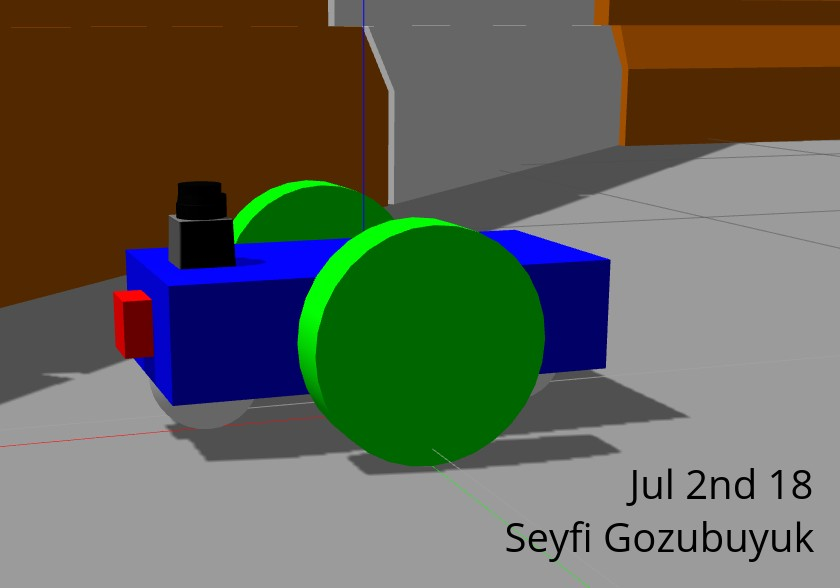
\includegraphics[width=\linewidth]{figures/UdacityBotGazebo.png}
      \caption{Udacity Bot in Gazebo}
      \label{fig:ubotgaz}
\end{figure}

\begin{figure}[thpb]
      \centering
      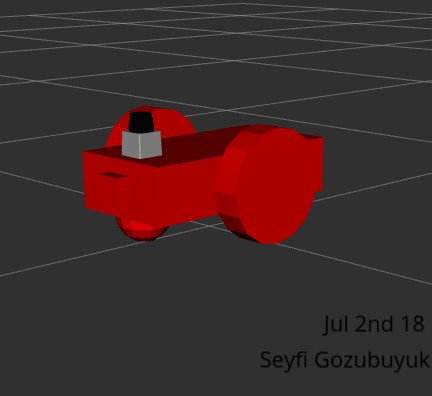
\includegraphics[width=\linewidth]{figures/UdacityBotRViz.png}
      \caption{Udacity Bot in RViz}
      \label{fig:ubotrvz}
\end{figure}

\subsection{The xbot}
The xbot is the slightly modified version of the Udacity Bot. It has a sensor base link which is in a rectangular box shape. This link is connected to the chassis and the laser sensor and the camera. Figure~\ref{fig:xbotgaz} and Figure~\ref{fig:xbotrvz} shows the xbot in Gazebo and RViz.

\begin{figure}[thpb]
      \centering
      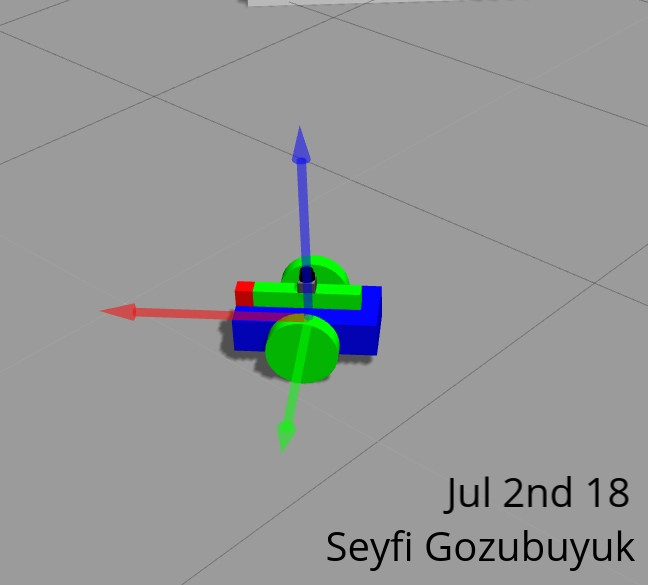
\includegraphics[width=\linewidth]{figures/xbotGazebo.png}
      \caption{xbot in Gazebo}
      \label{fig:xbotgaz}
\end{figure}

\begin{figure}[thpb]
      \centering
      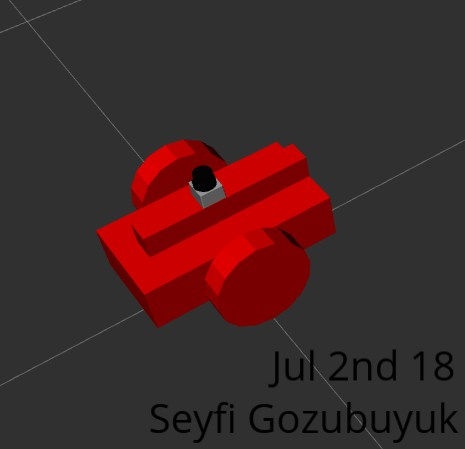
\includegraphics[width=\linewidth]{figures/xbotRViz.png}
      \caption{xbot in RViz}
      \label{fig:xbotrvz}
\end{figure}


\subsection{Achievements}
The Udacity bot and the xbot were able to reach the goal location. However, they first went in the opposite direction to find a way to goal. After recognizing there was no way to goal, they turned back and the reach to the target.

% Robot Models
\subsection{Benchmark Model}
\subsubsection{Model design}
The main part of the Udacity bot is the chassis. It has a box shape with dimensions 0.4 x 0.2 x 0.1. It has two casters, one at -0.15 0 -0.05 and the other at 0.15 0 -0.05. There are two wheels connected to the chassis at 0 -0.15 0 and 0 +0.15 0. //
The laser sensor located at position relative to the chassis 0.15 0 0.085. It has a cubic shape with length 0.1. The camera sensor is connected to the chassis at 0.2 0 0, and it has a cubic shape with lenght 0.05.

\subsubsection{Packages Used}
The packages used are as follows:
\begin{itemize}
\item ros-kinetic-navigation
\item ros-kinetic-map-server
\item ros-kinetic-move-base
\item ros-kinetic-amcl
\end{itemize}

Figure~\ref{fig:ubotgrp} and Figure~\ref{fig:xbotgrp} shows the topics for the Udacity Bot and the xbot.


\begin{figure}[thpb]
      \centering
      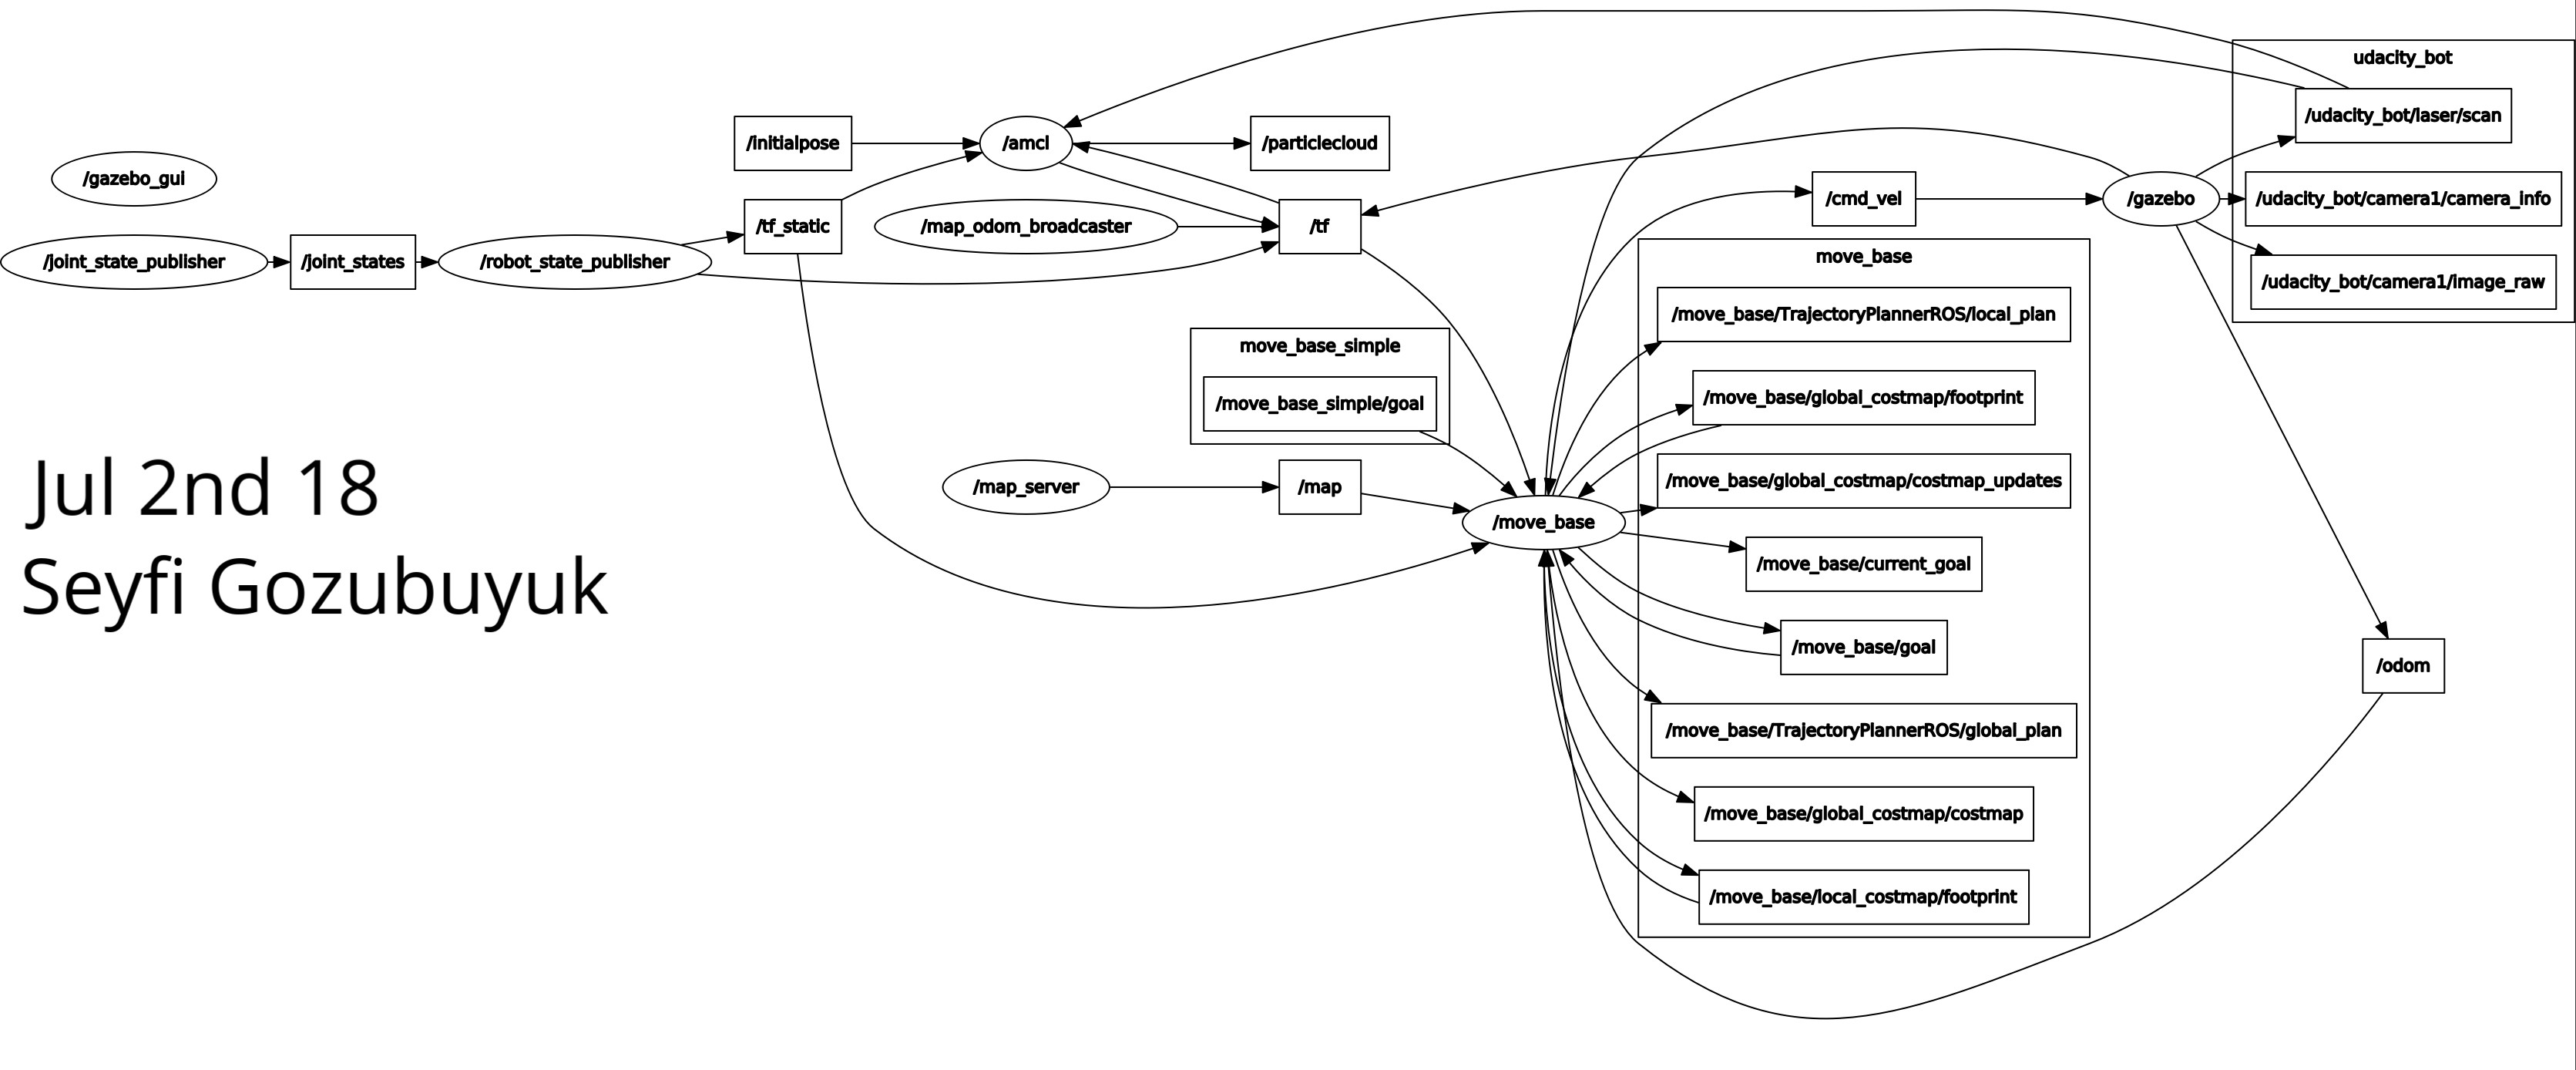
\includegraphics[width=\linewidth]{figures/rosgraph_ubot.png}
      \caption{Udacity Bot Rosgraph}
      \label{fig:ubotgrp}
\end{figure}

\begin{figure}[thpb]
      \centering
      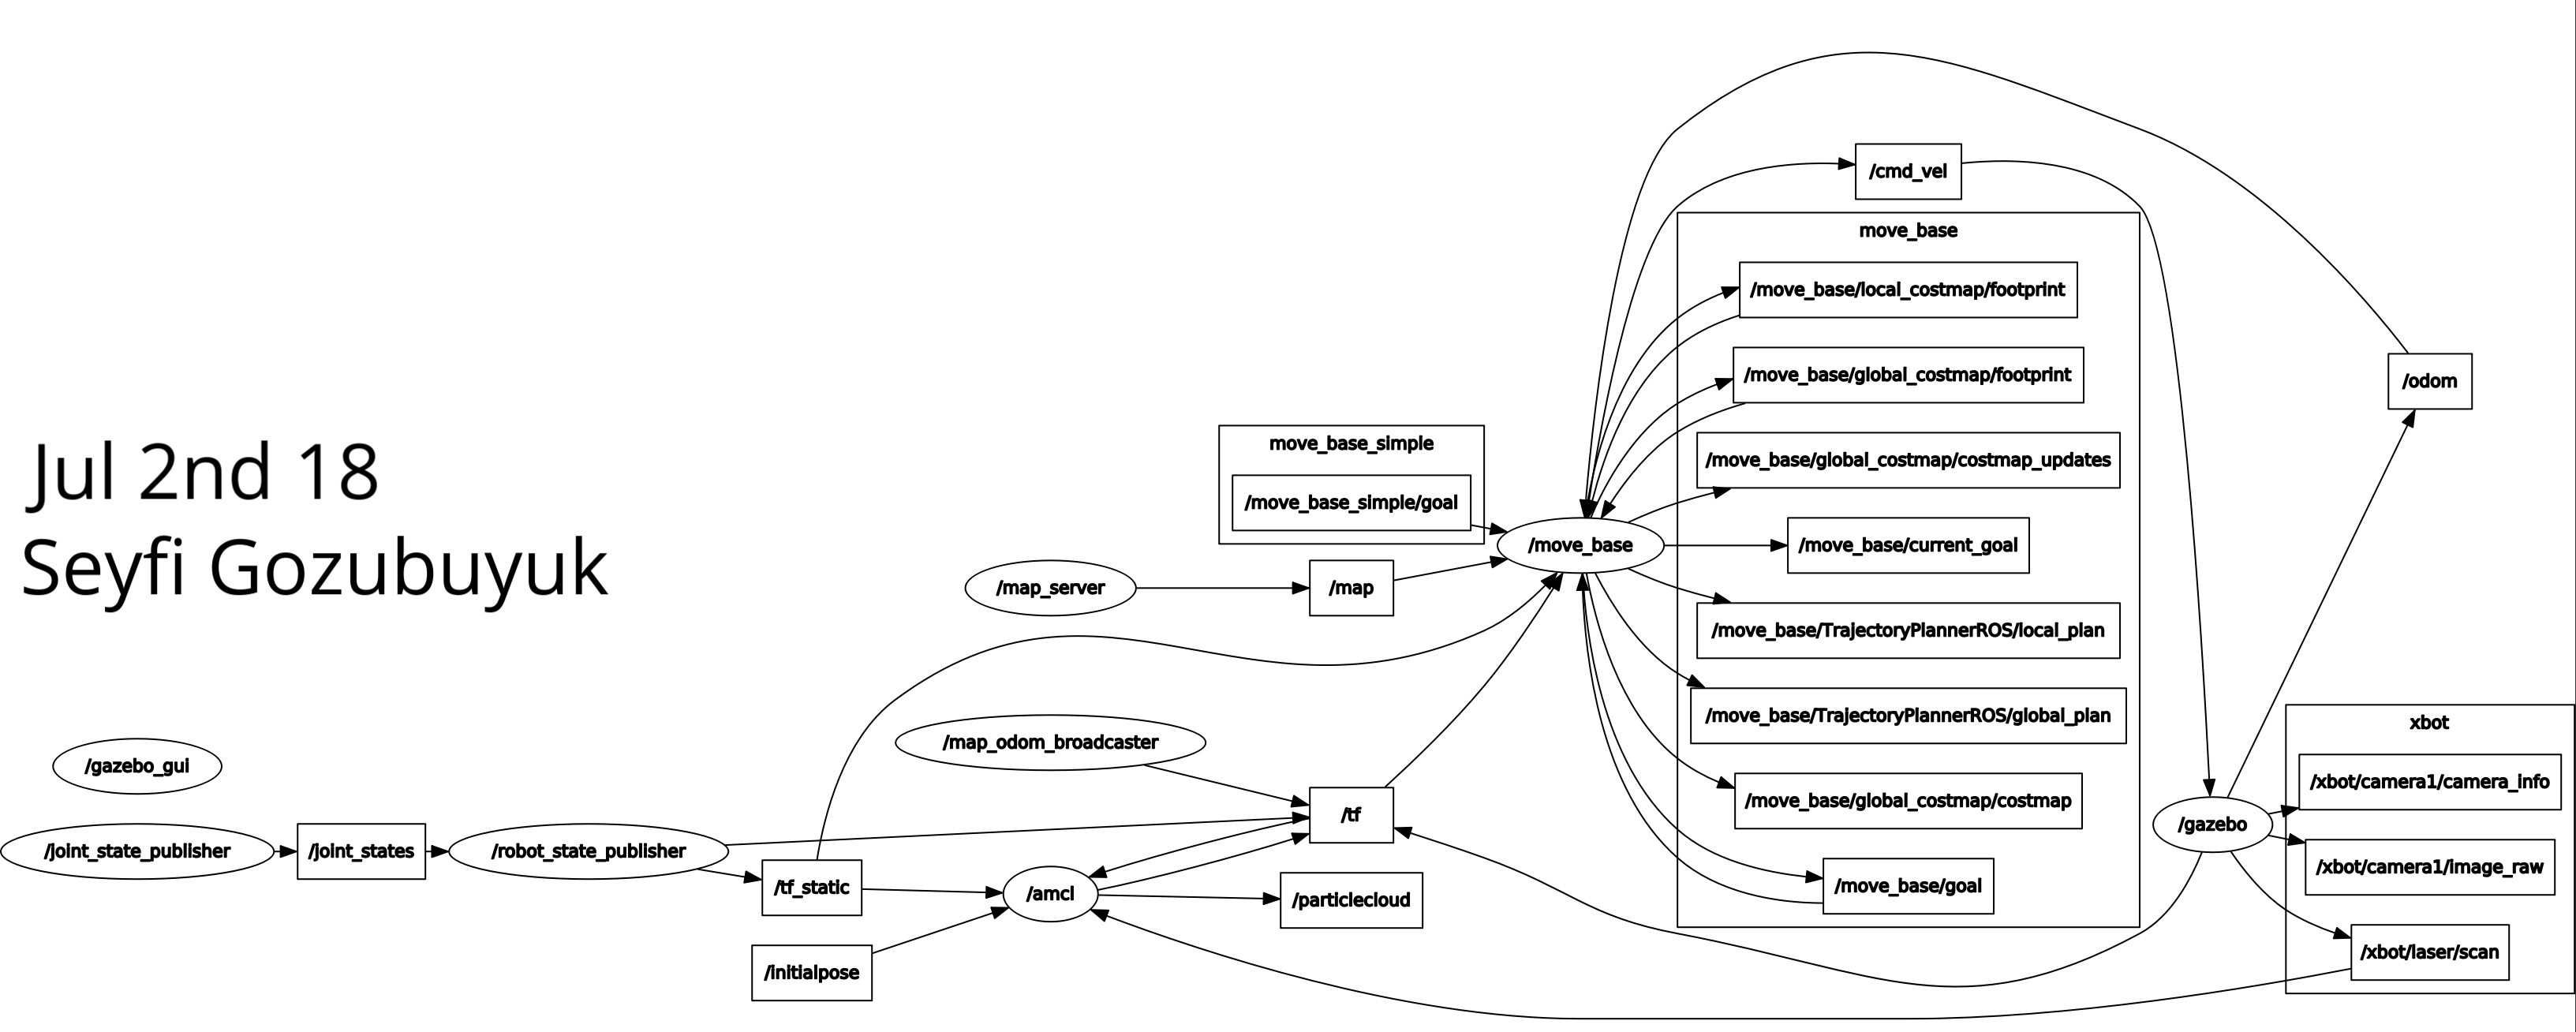
\includegraphics[width=\linewidth]{figures/rosgraph_xbot.png}
      \caption{xbot Rosgraph}
      \label{fig:xbotgrp}
\end{figure}



The packages used in the project should be specified as well as the topics received and published; the services it used and provided should also be addressed.

\subsubsection{Parameters}
Localization parameters in the AMCL node should be described, as well as move\_base parameters in the configuration file. You should be able to clearly demonstrate your understanding of the impact of these parameters.

\subsection{Personal Model}
% ditto
\subsubsection{Model design}
\subsubsection{Packages Used}
\subsubsection{Parameters}


\section{Results}
Present an unbiased view of your robot's performance and justify your stance with facts. Do the localization results look reasonable? What is the duration for the particle filters to converge? How long does it take for the robot to reach the goal? Does it follow a smooth path to the goal? Does it have unexpected behavior in the process? \\
For demonstrating your results, it is incredibly useful to have some watermarked charts, tables, and/or graphs for the reader to review. This makes ingesting the information quicker and easier.

\subsection{Localization Results}
\subsubsection{Benchmark}
\subsubsection{Student}

\subsection{Technical Comparison} % only facts
Discuss the difference of the layout, parameters, performance etc. between the benchmark robot and your robot. It is acceptable for your custom robot to perform worse than the provided robot. The focus is on learning and understanding, not performance.

\section{Discussion}
This is the only section of the report where you may include your opinion. However, make sure your opinion is based on facts. If your robot performed poorly, make mention of what may be the underlying issues. If the robot runs well, which aspects contribute to that? Again, avoid writing in the first person (i.e. Do not use words like "I" or "me"). If you really find yourself struggling to avoid the word "I" or "me"; sometimes, this can be avoid with the use of the word “one”. As an example: instead of : "I think the robot cannot localize itself because the sensor does not provide enough information for localization" try: "one may believe the localization performance is poor because the sensor layout is not able to provide enough information for localization". They say the same thing, but the second avoids the first person.

\subsection{Topics}
\begin{itemize}
\item Which robot performed better?
\item Why it performed better? (opinion)
\item How would you approach the 'Kidnapped Robot' problem?
\item What types of scenario could localization be performed?
\item Where would you use MCL/AMCL in an industry domain?
\end {itemize}

\section{Conclusion / Future work}
This section is intended to summarize your report. Your summary should include a recap of the results, did this project achieve what you attempted, how would you deploy it on hardware and how could this project be applied to commercial products?
For Future Work, address areas of work that you may not have addressed in your report as possible next steps. This could be due to time constraints, lack of currently developed methods / technology, and areas of application outside of your current implementation. Again, avoid the use of the first-person.

\subsection{Modifications for Improvement}
Examples:
\begin{itemize}
\item Base Dimension
\item Sensor Location
\item Sensor Layout
\item Sensor Amount
\end{itemize}

\subsection{Hardware Deployment}
\begin{enumerate}
\item What would need to be done?
\item Computation time/resource considerations?
\end{enumerate}



\bibliography{bib}
\bibliographystyle{ieeetr}

\end{document}